% Options for packages loaded elsewhere
\PassOptionsToPackage{unicode}{hyperref}
\PassOptionsToPackage{hyphens}{url}
%
\documentclass[
  8pt,
  ignorenonframetext,
]{beamer}
\usepackage{pgfpages}
\setbeamertemplate{caption}[numbered]
\setbeamertemplate{caption label separator}{: }
\setbeamercolor{caption name}{fg=normal text.fg}
\beamertemplatenavigationsymbolsempty
% Prevent slide breaks in the middle of a paragraph
\widowpenalties 1 10000
\raggedbottom
\setbeamertemplate{part page}{
  \centering
  \begin{beamercolorbox}[sep=16pt,center]{part title}
    \usebeamerfont{part title}\insertpart\par
  \end{beamercolorbox}
}
\setbeamertemplate{section page}{
  \centering
  \begin{beamercolorbox}[sep=12pt,center]{part title}
    \usebeamerfont{section title}\insertsection\par
  \end{beamercolorbox}
}
\setbeamertemplate{subsection page}{
  \centering
  \begin{beamercolorbox}[sep=8pt,center]{part title}
    \usebeamerfont{subsection title}\insertsubsection\par
  \end{beamercolorbox}
}
\AtBeginPart{
  \frame{\partpage}
}
\AtBeginSection{
  \ifbibliography
  \else
    \frame{\sectionpage}
  \fi
}
\AtBeginSubsection{
  \frame{\subsectionpage}
}
\usepackage{amsmath,amssymb}
\usepackage{lmodern}
\usepackage{ifxetex,ifluatex}
\ifnum 0\ifxetex 1\fi\ifluatex 1\fi=0 % if pdftex
  \usepackage[T1]{fontenc}
  \usepackage[utf8]{inputenc}
  \usepackage{textcomp} % provide euro and other symbols
\else % if luatex or xetex
  \usepackage{unicode-math}
  \defaultfontfeatures{Scale=MatchLowercase}
  \defaultfontfeatures[\rmfamily]{Ligatures=TeX,Scale=1}
\fi
\usetheme[]{metropolis}
% Use upquote if available, for straight quotes in verbatim environments
\IfFileExists{upquote.sty}{\usepackage{upquote}}{}
\IfFileExists{microtype.sty}{% use microtype if available
  \usepackage[]{microtype}
  \UseMicrotypeSet[protrusion]{basicmath} % disable protrusion for tt fonts
}{}
\makeatletter
\@ifundefined{KOMAClassName}{% if non-KOMA class
  \IfFileExists{parskip.sty}{%
    \usepackage{parskip}
  }{% else
    \setlength{\parindent}{0pt}
    \setlength{\parskip}{6pt plus 2pt minus 1pt}}
}{% if KOMA class
  \KOMAoptions{parskip=half}}
\makeatother
\usepackage{xcolor}
\IfFileExists{xurl.sty}{\usepackage{xurl}}{} % add URL line breaks if available
\IfFileExists{bookmark.sty}{\usepackage{bookmark}}{\usepackage{hyperref}}
\hypersetup{
  pdftitle={Class 10: Spatial Regression},
  pdfauthor={Jonathan Tannen},
  hidelinks,
  pdfcreator={LaTeX via pandoc}}
\urlstyle{same} % disable monospaced font for URLs
\newif\ifbibliography
\usepackage{graphicx}
\makeatletter
\def\maxwidth{\ifdim\Gin@nat@width>\linewidth\linewidth\else\Gin@nat@width\fi}
\def\maxheight{\ifdim\Gin@nat@height>\textheight\textheight\else\Gin@nat@height\fi}
\makeatother
% Scale images if necessary, so that they will not overflow the page
% margins by default, and it is still possible to overwrite the defaults
% using explicit options in \includegraphics[width, height, ...]{}
\setkeys{Gin}{width=\maxwidth,height=\maxheight,keepaspectratio}
% Set default figure placement to htbp
\makeatletter
\def\fps@figure{htbp}
\makeatother
\setlength{\emergencystretch}{3em} % prevent overfull lines
\providecommand{\tightlist}{%
  \setlength{\itemsep}{0pt}\setlength{\parskip}{0pt}}
\setcounter{secnumdepth}{-\maxdimen} % remove section numbering
\makeatletter
\def\mathcolor#1#{\@mathcolor{#1}}
\def\@mathcolor#1#2#3{%
  \protect\leavevmode
  \begingroup
    \color#1{#2}#3%
  \endgroup
}
\makeatother

\definecolor{sixtysix_red}{HTML}{FF5675}
\setbeamercolor{title separator}{fg=sixtysix_red}
\ifluatex
  \usepackage{selnolig}  % disable illegal ligatures
\fi

\title{Class 10: Spatial Regression}
\author{Jonathan Tannen}
\date{}

\begin{document}
\frame{\titlepage}

\begin{frame}{Agenda}
\protect\hypertarget{agenda}{}
\begin{itemize}
\tightlist
\item
  Spatial Regressions
\item
  Mid-Point Presentations
\end{itemize}
\end{frame}

\begin{frame}{Looking Ahead}
\protect\hypertarget{looking-ahead}{}
Next Week: Code Review (or Implementation Review) for two projects.
Phila Dept of Public Health Presenting.

April 8: World Resources Institute Presenting.

April 15/22: Final Presentations

April 29: Final Project Due
\end{frame}

\begin{frame}{High-Level notes from Mid-Points}
\protect\hypertarget{high-level-notes-from-mid-points}{}
\begin{itemize}
\tightlist
\item
  Use the Literature Review to help the reader understand why your topic
  is important.

  \begin{itemize}
  \tightlist
  \item
    Include the \emph{findings} of the papers.
  \end{itemize}
\item
  Do a lot explaining the \emph{why} behind your methods.

  \begin{itemize}
  \tightlist
  \item
    What is the purpose of your controls?
  \item
    What is the challenge in your risk score?
  \end{itemize}
\item
  Include a lot more summary stats and overall plots of your data.

  \begin{itemize}
  \tightlist
  \item
    Don't jump into regression too soon!
  \end{itemize}
\end{itemize}
\end{frame}

\begin{frame}{Spatial Regressions}
\protect\hypertarget{spatial-regressions}{}
Consider the linear regression equation:

\[Y = X\beta + \epsilon\] \pause

\begin{itemize}
\tightlist
\item
  \(\epsilon\) contains all unobserved variables not in \(X\).
\item
  Estimation requires the following (strong) assumptions\ldots{}

  \begin{itemize}
  \tightlist
  \item
    \(E[\epsilon | X] = 0\)

    \begin{itemize}
    \tightlist
    \item
      aka \(\epsilon\) is not independent of \(X\).
    \item
      Introduces ``Omitted Variable Bias''. \pause
    \end{itemize}
  \item
    \(Cov(\epsilon_i, \epsilon_j) = 0\)

    \begin{itemize}
    \tightlist
    \item
      When this is due to \(i\) and \(j\) being close, this is spatial
      autocorrelation.
    \item
      You actually have fewer observations than you think.
    \end{itemize}
  \end{itemize}
\end{itemize}
\end{frame}

\begin{frame}{Spatial Regressions}
\protect\hypertarget{spatial-regressions-1}{}
Consider an example: Trying to predict the sales price of a house.

\[Y = X\beta + \epsilon\]

\begin{itemize}
\tightlist
\item
  What would be good to include in \(X\)? \pause
\item
  Suppose we only used features of the house as \(X\). Would the
  epsilons be correlated? Why?
\end{itemize}
\end{frame}

\begin{frame}{Spatial Regressions}
\protect\hypertarget{spatial-regressions-2}{}
\[Y = X\beta + \epsilon\]

What are the solutions to spatial autocorrelation?

The answer hinges on whether you care about (a) estimating coefficients
correctly, or (b) getting good predictions.

The three options:

\begin{itemize}
\tightlist
\item
  Introduce features that explain away the spatial correlation.
\item
  Aggregate up to a granularity at which there is no spatial
  correlation.
\item
  Use a fancy regression technique that corrects standard errors for
  autocorrelation.
\end{itemize}
\end{frame}

\begin{frame}{What is your unit of analysis?}
\protect\hypertarget{what-is-your-unit-of-analysis}{}
\begin{itemize}
\tightlist
\item
  Points
\item
  Polygons
\end{itemize}

\pause

This has implications for\ldots{}

\begin{itemize}
\tightlist
\item
  What you control for (and how).
\item
  How you specify spatial covariances.
\end{itemize}
\end{frame}

\begin{frame}{Estimating Coefficients}
\protect\hypertarget{estimating-coefficients}{}
Consider an example: Trying to predict the sales price of a house.

\[Y = X\beta + \epsilon\]

``What is the value of adding air conditioning?''

\begin{itemize}
\tightlist
\item
  What is the \(X\) we care about?
\item
  Why would \(\epsilon\) be correlated with it?
\item
  What should we control for?
\end{itemize}

\pause

All we care about is ``controlling away'' the spatial correlations.
\end{frame}

\begin{frame}{Diagnosing Autocorrelation}
\protect\hypertarget{diagnosing-autocorrelation}{}
\[Y = X\beta + \epsilon\]

Once we fit this model, is there evidence that
\(Cov(\epsilon_i, \epsilon_j)\) depends on distance?

\begin{itemize}
\item
  \textbf{Variogram}: Plot the covariance between values as a function
  of distance.
\item
  \textbf{Moran's I}:
  \(\hat{Cov}_W(\epsilon_i, \epsilon_j) / \hat{Cov(epsilon)}\)
\end{itemize}
\end{frame}

\begin{frame}[fragile]{Estimating Coefficients}
\protect\hypertarget{estimating-coefficients-1}{}
Consider an example: Trying to predict the sales price of a house.

\[Y = X\beta + \epsilon\]

Solutions:

\begin{itemize}
\tightlist
\item
  Add controls that explain the spatial correlation.

  \begin{itemize}
  \tightlist
  \item
    Proximity to schools? Neighborhood parks?
  \item
    Question: Should we control for median income? \pause
  \end{itemize}
\item
  Use ``Fixed Effects'' (e.g.~at Census Tracts) to blanket control for
  spatial patterns.

  \begin{itemize}
  \tightlist
  \item
    Add a dummy variable for each Census Tract.
  \item
    \(Y = X\beta + \gamma_0 \delta_0 + \gamma_1 \delta_1 + ... + \epsilon\)
  \item
    Pros: Blanket tool to control for unobserved variables that vary
    within tracts.
  \item
    Cons:

    \begin{itemize}
    \tightlist
    \item
      Limits analysis to only within-tract comparisons. \pause
    \end{itemize}
  \end{itemize}
\item
  Random Effects, or Hierarchical Model

  \begin{itemize}
  \tightlist
  \item
    Allows you to add tract-level variables, estimates standard errors
    correctly.
  \item
    \(Y = X\beta + \gamma Z_{Tract} + \epsilon\)
  \item
    in R: \texttt{rmle} package.
  \end{itemize}
\end{itemize}
\end{frame}

\begin{frame}{Aggregating up to higher level of granularity}
\protect\hypertarget{aggregating-up-to-higher-level-of-granularity}{}
Consider an example: Trying to predict the sales price of a house.

\[Y = X\beta + \epsilon\]

``What is the value of a school?''

\begin{itemize}
\tightlist
\item
  What is the \(X\) we care about?
\item
  Why would \(\epsilon\) be correlated with it?
\item
  What should we control for?
\end{itemize}

\pause

All schools in a given catchment will receive the same school effect. Do
analysis at the \emph{school level} rather than the house level.
\end{frame}

\begin{frame}[fragile]{True autocorrelation: Smarter Regression Models}
\protect\hypertarget{true-autocorrelation-smarter-regression-models}{}
Consider an example: Trying to predict the sales price of a house.

\[Y = X\beta + \epsilon\]

Solution: Methods that simultaneously check and remove autocorrelation.

\begin{itemize}
\tightlist
\item
  Simultaneous Auto Regression (SAR) and Conditional Auto Regression
  methods.
\item
  package \texttt{spatialreg} in R.
\end{itemize}
\end{frame}

\begin{frame}{Crime in Philadelphia (McClellan 2022)}
\protect\hypertarget{crime-in-philadelphia-mcclellan-2022}{}
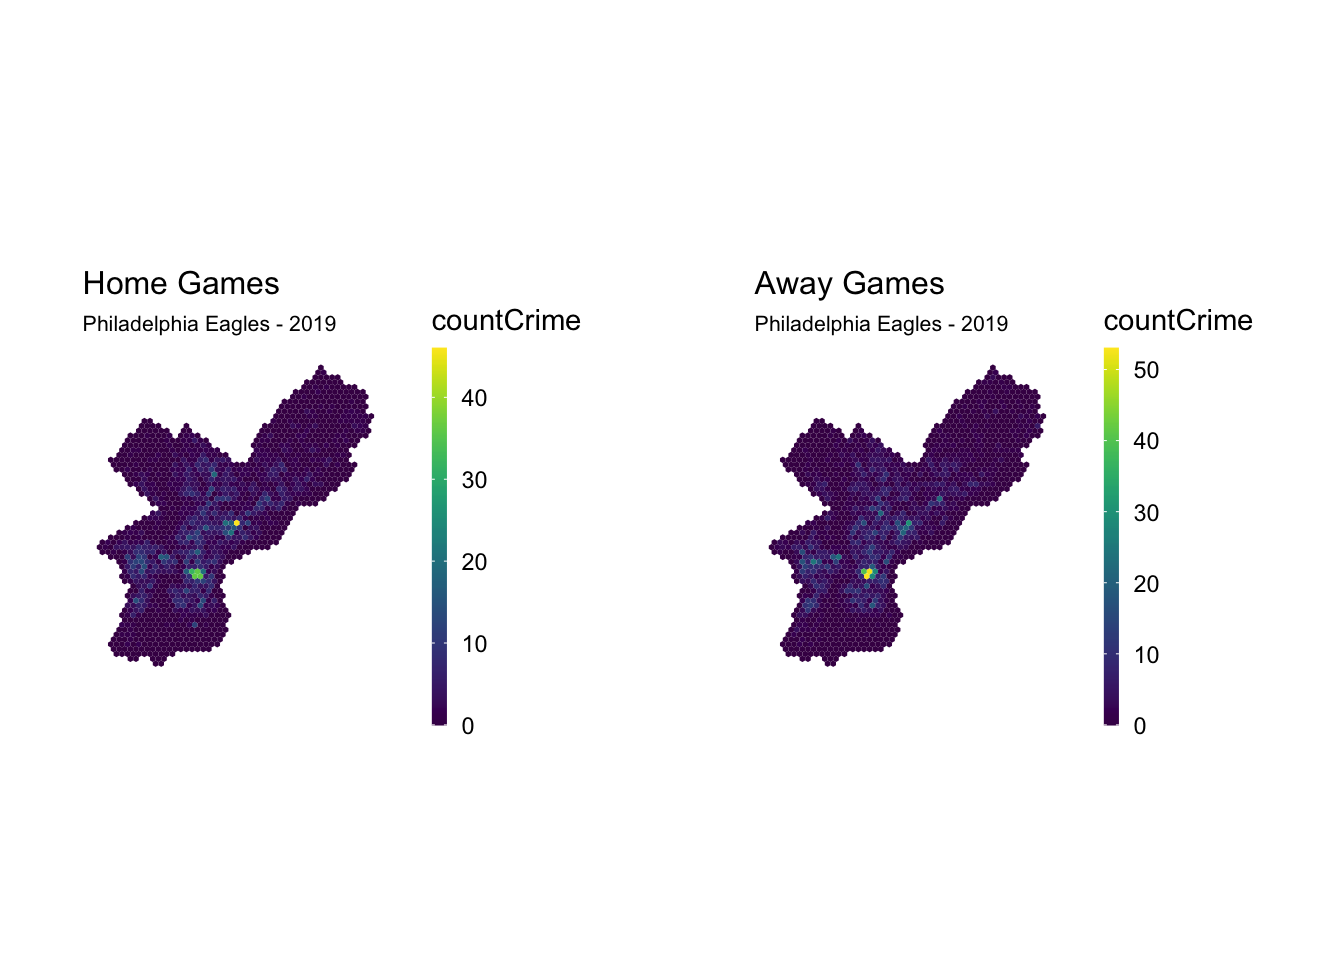
\includegraphics[width=0.8\textwidth,height=\textheight]{images/crime_plots.png}

\begin{itemize}
\tightlist
\item
  Is there spatial autocorrelation?
\item
  Is there omitted variable bias?
\item
  How should we control spatial unobserved features?
\end{itemize}

\pause

\[
crime = \alpha + \beta_0 anygame + \beta_1 homegame * anygame + \beta_2 Z + \epsilon
\]
\end{frame}

\begin{frame}{Demo}
\protect\hypertarget{demo}{}
\end{frame}

\begin{frame}{Mid-Point Presentations}
\protect\hypertarget{mid-point-presentations}{}
Room A: Here Room B: 323

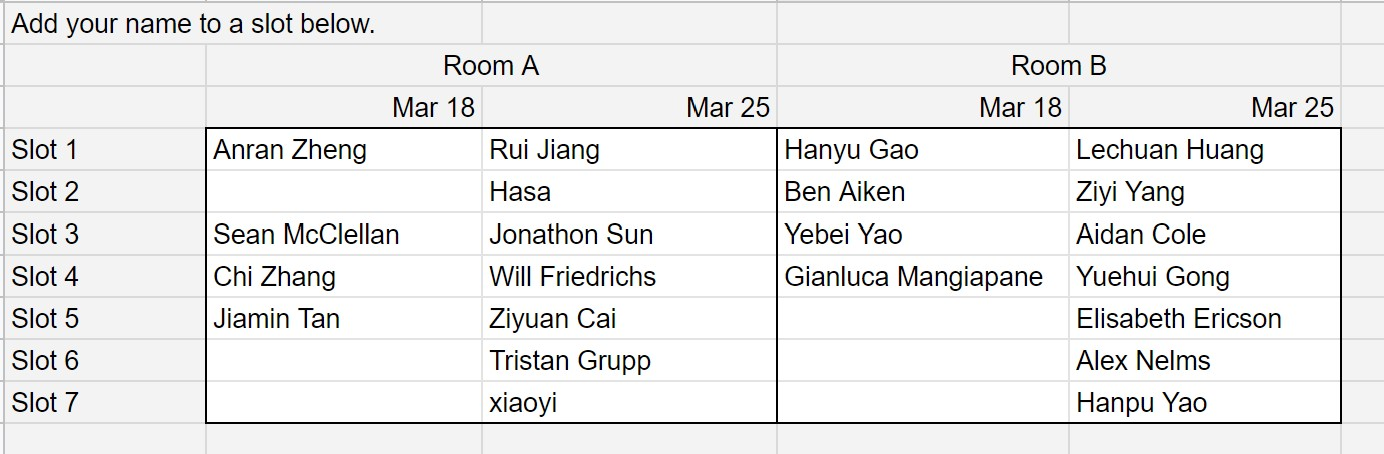
\includegraphics{images/midpoint_schedule_20220325.jpg}
\end{frame}

\end{document}
